\documentclass{article}
\usepackage[utf8]{inputenc} %кодировка
\usepackage[T2A]{fontenc}
\usepackage[english,russian]{babel} %русификатор
\usepackage{mathtools} %библиотека матеши
\usepackage[left=1cm,right=1cm,top=2cm,bottom=2cm,bindingoffset=0cm]{geometry} %изменение отступов на листе
\usepackage{amsmath}
\usepackage{graphicx} %библиотека для графики и картинок
\graphicspath{}
\DeclareGraphicsExtensions{.pdf,.png,.jpg}
\usepackage{subcaption}
\usepackage{pgfplots}
\usepackage{array}
\usepackage{pgfplots}
\pgfplotsset{compat=1.16}

\begin{document}
% НАЧАЛО ТИТУЛЬНОГО ЛИСТА
\begin{center}
    \Large
    Федеральное государственное автономное \\
    образовательное учреждение высшего образования \\
    «Научно-образовательная корпорация ИТМО»\\
    \vspace{0.5cm}
    \large
    Факультет программной инженерии и компьютерной техники \\
    Направление подготовки 09.03.04 Программная инженерия \\
    \vspace{1cm}
    \Large
    \textbf{Отчёт по лабораторной работе №1} \\
    По дисциплине «Математическая статистика» (четвёртый семестр)\\
    Исследование распределения случайной величины\\
    \large
    \vspace{8cm}

    \begin{minipage}{.33\textwidth}
    \end{minipage}
    \hfill
    \begin{minipage}{.4\textwidth}

        \textbf{Студент}: \vspace{.1cm} \\
        \ Билошицкий Михаил Владимирович\\
        \ Беляев Михаил Сергеевич\\
        \ Сиразетдинов Азат Ниязович\\
        \textbf{Преподаватель}:  \\
        \ Милованович Екатерина Воиславовна
    \end{minipage}
    \vfill
Санкт-Петербург\\ 2024 г.
\end{center}

% КОНЕЦ ТИТУЛЬНОГО ЛИСТА
\newpage
\section*{Цель работы:}
\large

На основании анализа опытных данных

1. Построить интервальный ряд; полигон частот; выборочную функцию распределения; гистограмму для изучения признака

2. Вычислить точечные оценки математического ожидания и дисперсии

3. Построить доверительные интервалы для мат ожидания и дисперсии с доверительной вероятностью 0,95

% 4. Проверить статистическую гипотезу о виде закона распределения генеральной совокупности.
\section{Интервальный ряд}
По условию нам дано n = 100. Получим k - число интервалов:
\begin{equation}
    k = \sqrt{n}
\end{equation}
\begin{equation*}
    k = \sqrt{100} = 10
\end{equation*}
Таблица для оценивания исследования распределения случайной величины:
\begin{table}[h]
    \centering
    \begin{tabular}{|*{10}{c|}}
        \hline
        0.866 & -0.005 & 0.403 & 1.908 & 0.448 & 0.169 & -0.731 & -1.189 & 0.905 & 0.283 \\
        \hline
        2.431 & 1.409 & 0.191 & -0.165 & 0.889 & 0.804 & -2.131 & -0.754 & 1.458 & 1.650 \\
        \hline
        0.110 & 1.757 & -0.693 & -0.732 & 1.073 & -1.724 & -1.810 & 0.947 & -1.118 & 0.666 \\
        \hline
        0.026 & 0.885 & 0.011 & -0.990 & -0.104 & 0.174 & -0.052 & -0.182 & 1.813 & 0.346 \\
        \hline
        0.970 & 1.140 & -1.105 & 0.894 & 1.547 & -0.484 & -0.086 & -0.066 & 0.150 & -0.264 \\
        \hline
        0.350 & 0.033 & 0.478 & 0.637 & -0.033 & -0.319 & 0.570 & -0.837 & -0.413 & -1.640 \\
        \hline
        -0.795 & -0.015 & 1.774 & -1.568 & 0.302 & -1.120 & -0.917 & -0.091 & 1.118 & 0.277 \\
        \hline
        -0.622 & -0.554 & -0.470 & 0.700 & -0.656 & 1.460 & 1.701 & 0.630 & -0.700 & -0.674 \\
        \hline
        1.429 & -1.163 & -0.925 & 0.973 & -0.052 & 0.409 & -0.024 & 0.384 & -0.350 & 0.203 \\
        \hline
        -2.084 & 0.100 & 0.001 & -0.070 & 0.773 & 1.132 & -0.769 & -0.609 & 1.816 & 1.307 \\
        \hline
    \end{tabular}
    \caption{Данные}
\end{table}
\\
Для выборки min = -2.131, max = 2.431.
Для удобства расчётов пусть min = -2.15, max = 2.45
\begin{equation*}
    a_{min} = -2.15;\ \  b_{max} = 2.45
\end{equation*}
По формуле найдём шаг разбиения:
\begin{equation}
    h = \frac{b-a}{k}
\end{equation}
\begin{equation*}
    h = \frac{4.6}{10} = 0.46
\end{equation*}
Введём отрезок $[a,\ b]$, длина которого $10h$. Разбиваем его на 10 равных частичных интервалов, определяем частоты и относительные частоты. Представитьеля каждого интервала будем считать по формуле:
\begin{equation}
    x_i^* = \frac{x_{i-1}+x_i}{2}
\end{equation}

\begin{table}[h]
    \scriptsize
    \begin{tabular}{|*{11}{c|}}
        \hline
        Номер & 1  & 2  & 3  & 4  & 5  & 6  & 7  & 8  & 9  & 10 \\
        \hline
        Интервалы &[-2.15, -1.67) & \tiny[-1.67, -1.22) & \tiny[-1.22, -0.76) & \tiny[-0.76, -0.31) & \tiny[-0.31, 0.15) & \tiny[0.15, 0.61) & \tiny[0.61, 1.06) & \tiny[1.06, 1.52) & \tiny[1.52, 1.97) & \tiny[1.97, 2.45) \\
        \hline
        $x_i^*$& -1.91 & -1.45 & -0.99 & -0.53 & -0.08 & 0.38 & 0.83 & 1.29 & 1.75 & 2.21\\
        \hline
        $m_i$& 4 & 2 & 11 & 15 & 20 & 16 & 14 & 9 & 8 & 1	\\
        \hline
        $p_i^*$& 0.04 & 0.02 & 0.11 & 0.15 & 0.20 & 0.16 & 0.14 & 0.09 & 0.08 & 0.01\\
        \hline
        $h_i$& 0.09 & 0.04 & 0.24 & 0.33 & 0.44 & 0.35 & 0.31 & 0.20 & 0.18 & 0.02 \\
        \hline
    \end{tabular}
    \caption{Интервальный ряд с характеристиками}
\end{table}

\[h_i = \frac{p_i^*}{h}\]
\begin{figure}[h!]
    \begin{center}
    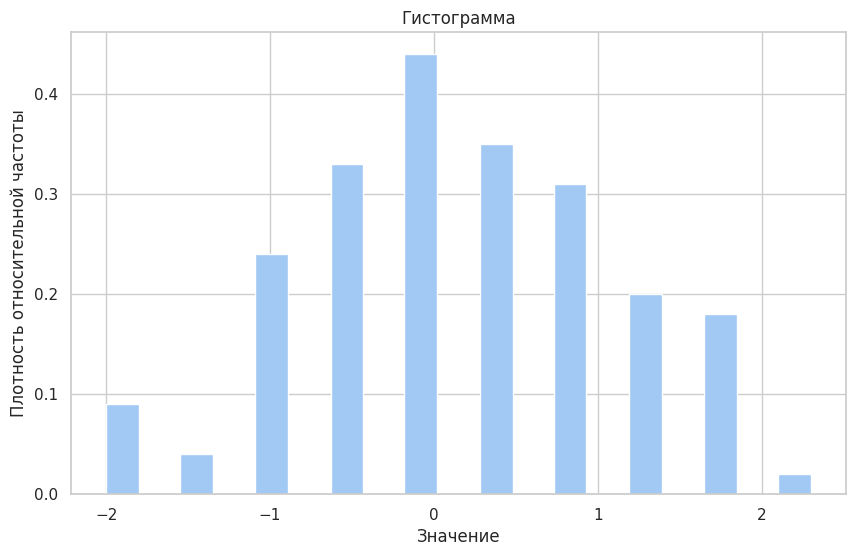
\includegraphics[width=.7\textwidth]{hist}
    \caption{\small Гистограмма}
    \end{center}
    \begin{center}
    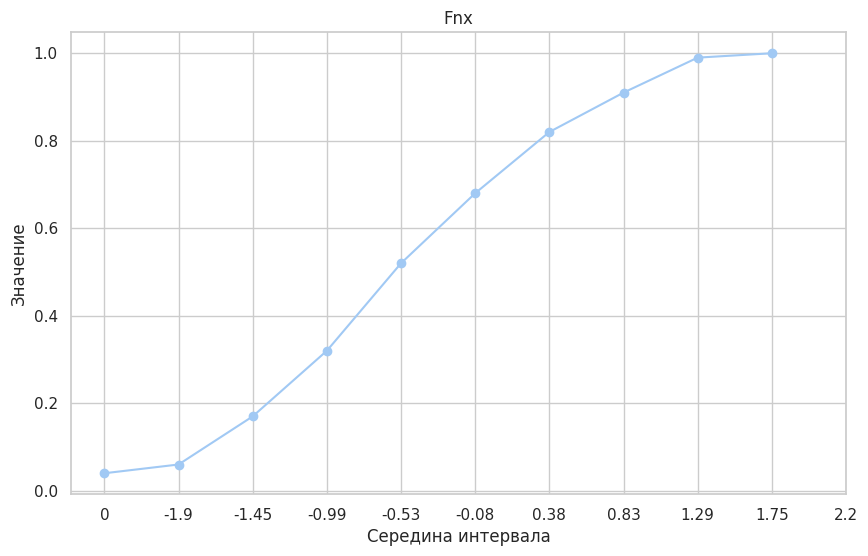
\includegraphics[width=.7\textwidth]{function}
    \caption{\small Эмпирическая функция распределения}
    \end{center}
\end{figure}



\newblock
\section{Вычисление точечных оценок мат ожидания и дисперсии}
Найдем точечные оценки математического ожидания и дисперсии. В качестве таких оценок выбирают среднее выборочное значение:
\[\overline{X} = \sum_{i=1}^{10}x_i^*p_i^*\]
и выборочную дисперсию:
\[S^2 = \sum_{i=1}^{10}(x_i^* - \overline{X})^2p_i^* = \sum_{i=1}^{10}x_i^{*2}p_i^* - \overline{X}^2 = m_2 - \overline{X}^2\]
где
\[m_2 = \sum_{i=1}^{10}x_i^{*2}p_i^*\]
\begin{table}[h]
    \begin{tabular}{|*{12}{c|}}
        \hline
        Номер & 1  & 2  & 3  & 4  & 5  & 6  & 7  & 8  & 9  & 10& некоторые рез-ты \\
        \hline
        $x_i^*$& -1.91 & -1.45 & -0.99 & -0.53 & -0.08 & 0.38 & 0.83 & 1.29 & 1.75 & 2.21 & -\\
        \hline
        $p_i^*$& 0.04 & 0.02 & 0.11 & 0.15 & 0.20 & 0.16 & 0.14 & 0.09 & 0.08 & 0.01& -\\
        \hline
        $x_i^{*}p_i^*$& -0.076 & -0.029 & -0.109 & -0.08 & -0.016 & 0.061 & 0.116 & 0.116 & 0.14 & 0.022 & 0.145\\
        \hline
        $x_i^{*2}p_i^*$& 0.146 & 0.042 & 0.108 & 0.042 & 0.001 & 0.023 & 0.096 & 0.15 & 0.245 & 0.049 & 0.902\\
        \hline
    \end{tabular}
    \caption{Данные для подсчёта мат ожидания и дисперсии}
\end{table}
\\
Оценка математического ожидания: 0.145\\
Оценка дисперсии: 0.881
\newblock

\section{Построить доверительные интервалы для мат ожидания и дисперсии}
Для рассматриваемого примера будем иметь:
\[\gamma = 0,95;\]
тогда находим по таблице распределения Стьюдента для 0.05 квантиль  t = 2.262, поэтому в нашем примере имеем:
\[\overline{X}-t\frac{S}{\sqrt{n}} = 0.145 - 2.262 \cdot\frac{\sqrt{0.881}}{\sqrt{10}} = -0.15\]
\[\overline{X}+t\frac{S}{\sqrt{n}} = 0.145 + 2.262 \cdot\frac{\sqrt{0.881}}{\sqrt{10}} = 0.44\]
таким образом:
\[-0.15 < m < 0.44\]
Для дисперсии определим квантили распределения хи-квадрат с 9 степенями свободы:
\[
\chi^2_{1-\alpha/2, n-1} = \chi^2_{1-\frac{0.05}{2}, 9} = \chi^2_{0.975, 9} = 2.7
\]
\[
\chi^2_{\alpha/2, n-1} = \chi^2_{0.025, 9} = 19.02
\]
По формуле подставим:
\[
\left(\frac{{(n-1)s^2}}{{\chi^2_{\alpha/2, n-1}}}, \frac{{(n-1)s^2}}{{\chi^2_{1-\alpha/2, n-1}}} \right)
\]
\[
\left( \frac{{9\cdot 0.881}}{19.02 }, \frac{{9\cdot 0.881}}{2.7} \right)
\]
Доверительный интервал для дисперсии:
\[ 0.416 < s^2 < 2.93\]
\section*{Вывод}
На основании анализа опытных данных: построили интервальный ряд; полигон частот; выборочную функцию распределения; гистограмму для изучения признака.
Вычислили точечные оценки мат ожидания и дисперсии.
Построили доверительные интервалы для мат ожидания и дисперсии с доверительной вероятностью 0,95.
\end{document}
\includegraphics[width=.9\textwidth]{123}